%!TEX encoding=UTF-8 Unicode
\chapter{Memory Performance Analysis}

The results of our case study (\chap{perf}) showed that traditional performance analysis tools can help identify memory related performance issues.
Yet they are not able to tell precisely where, in terms of data structures, the issue occurs.
Thus it is still required to analyze the code manually.
As memory is often a performance bottleneck, several tools where developed to analyze performance in regards of the memory.

This chapter discuss memory analysis tools, first we present the specificities of recent memory subsystems and the usual mistakes that can generate performances drop in \sect{archi}.
Then we present existing memory performance analysis tools and discuss their limitation in \sect{mem-tools}.
Finally we describe what would be in idealistic memory performance analysis tool \sect{mem-cncl}.

\section{Architectural considerations}
\label{sec:archi}

During a few decades, processor frequency increased significantly more than memory frequencies, resulting in a considerable gap between these two resources.
Retrieving one piece of data cost around $180$ \gls{CPU} cycles~\cite{Levinthal09Performance}.
Nevertheless most applications reuse most of their data.
Moreover during a small piece of time, a program usually work on a small set of data.
Hence \glspl{CPU} embed some caches to reduce the number of accesses actually generating a fetch from the main memory.
These caches are organized hierarchically, thus, the time required to access a piece of data depends on the cache level in which it is present.
One access to the fastest cache usually cost about $4$ \gls{CPU} cycles.
As these caches are small, every time a data is added in a cache it replaces (evict) an existing one.
Several mechanisms where designed to guess which data should be in the cache and which one should be evicted.
As a result, a developer seeking for performances must consider the architecture of these caches and the way the work to benefit from them.

\subsection{Memory Caches}

% Locality
There are two phenomena called \emph{spatial locality} and \emph{temporal locality} that can be observed in most programs and that are the main principles used for cache optimization.
Spatial locality is the fact that most programs do not usually access the memory in a completely random way, but they usually access data that are near to each other in a small chunk of time.
Similarly, temporal locality is the fact that a memory address is often used several times during a small interval of time.
Consequently the main role of caches is to keep data that have already been accessed close to the \gls{CPU} when they are reused to reduce the number of actual memory accesses.

\subsubsection{Cache lines and alignment}

To benefit even more from temporal locality, the memory is divided on lines (usually \SI{64}{bytes}), and every time an address must be fetched from the main memory, the whole line is copied to the cache.
Therefore accessing $8$ successive doubles (usually one double equals \SI{8}{bytes}) requires only one memory access if they all are in the same line of cache.
As a result, aligning data structure to cache line can improve the memory access time.

\begin{figure}[htb]
    \centering
    %!TEX encoding=UTF-8 Unicode
%Palette PurOr 4 Col
\definecolor{ColG}{HTML}{5E3C99}
\definecolor{ColB}{HTML}{FDB863}

\newcommand{\colg}[1]{\textcolor{ColG}{#1}}
\newcommand{\colb}[1]{\textcolor{ColB}{#1}}

\pgfdeclarelayer{bg}
\pgfsetlayers{bg,main}


\tikzstyle{arr}   = [-latex,thick]
\tikzstyle{txtnode} = [anchor=west]
\tikzstyle{mybrace} = [decorate,decoration={brace, mirror,amplitude=1em},thick]
\tikzstyle{mydash} = [dashed, dash pattern=on 1pt off 2pt]

\def\eltsz{3}
\def\vshift{-1.5}
\def\balign{.6}
\pgfmathparse{\balign*\eltsz}
\edef\balignsz{\pgfmathresult}
\def\nlines{1}
\pgfmathparse{\nlines-\balign}
\edef\resid{\pgfmathresult}

\tikzset{
    myarray/.style args={#1#2#3#4}{
        % args: size-1, fill, show number ?
        alias=this,
        append after command = {
            \pgfextra{
                \coordinate (#4-base) at ($(this.west)+(0,\vshift)$);
                \pgfmathparse{#1-1}
                \foreach \i in {0,...,\pgfmathresult}{
                    \draw[fill=#2] ($(#4-base)+(\eltsz*\i,0)$) rectangle ($(#4-base)+(\eltsz*\i+\eltsz,1)$);
                    \ifthenelse{#3=0}{}{
                        \node[anchor=south] at ($(#4-base)+(\eltsz*\i,1)$) {\i};
                    }
                }
                \ifthenelse{#3=0}{}{
                    \node[anchor=south] at ($(#4-base)+(\eltsz*#1,1)$){#1};
                }
            }
        }
    },
}



\begin{tikzpicture}[font=\small]
    \node[myarray={4}{none}{1}{bad},txtnode] (bad) at (0,0) {\colb{\textbf{Bad alignment:}}};

    \begin{pgfonlayer}{bg}
        \node[myarray={2}{ColG,mydash}{0}{invb},txtnode] (d0) at (\balignsz,0) {};
        \path[pattern=north east lines, pattern color=ColB] (0,\vshift) rectangle ($(0,\vshift)+(\balignsz,1)$);
        \path[pattern=north east lines, pattern color=ColB] (\balignsz+\eltsz*2,\vshift) rectangle (3*\eltsz,1+\vshift);
    \end{pgfonlayer}

    \draw[mybrace] (0,\vshift) -- (1*\eltsz,\vshift) node [midway,below=1em]
        {Fetch 0};
    \draw[mybrace] (\eltsz,\vshift) -- (2*\eltsz,\vshift) node [midway,below=1em]
        {Fetch 1};

    \draw[mybrace] (2*\eltsz,\vshift) -- (3*\eltsz,\vshift) node [midway,below=1em]
        {Fetch 2};

    \node[anchor=west] at (0,2*\vshift)
    {\textbf{Total:} \colb{3 fetches}, \colg{2~useful lines} / \colb{1~useless line}};

    %% Good alignment
    \node[myarray={4}{none}{1}{good},txtnode] (good) at (0,3*\vshift) {\colg{\textbf{Good alignment:}}};

    \begin{pgfonlayer}{bg}
        \node[myarray={2}{ColG,mydash}{0}{invg},txtnode] (d1) at (0,3*\vshift) {};
    \end{pgfonlayer}

    \draw[mybrace] (0,\vshift+3*\vshift) -- (\eltsz,\vshift+3*\vshift) node
        [midway,below=1em] {Fetch 0};
    \draw[mybrace] (\eltsz,\vshift+3*\vshift) -- (2*\eltsz,\vshift+3*\vshift) node
        [midway,below=1em] {Fetch 1};
    \node[anchor=west] at (0,5*\vshift)
    {\textbf{Total:} \colg{2 fetches}, \colg{2~useful lines} / \colb{0~useless lines}};

\end{tikzpicture}
% vim: et si sta lbr  sw=4 ts=4 spelllang=en_us

    \caption[Example of bad alignment.]{Retrieving two lines of cache with one or two fetches depending on the alignment of the lines.}
    \label{fig:bad-align}
\end{figure}

For instance if we consider accessing an array of two lines of caches as illustrated in \fig{bad-align}.
If the data structure is aligned to cache lines, it will take two accesses to retrieve the whole data structure, and no unused data will be introduced in the cache.
While if it is not correctly aligned, not only one more memory fetch will be required but we will introduce one useless line inside the cache.
As caches are designed to keep only a restricted number of data, inserting on line inside a cache means evicting another one, thus, introducing unused data must be avoided as much as possible.

\subsubsection{Cache management policies}

When an address is accessed, the \gls{CPU} must search for the corresponding line in the cache.
If it is not present, fetch it from the memory and decide where to copy it into the cache, which means choosing one line to evict.
To make the cache efficient, these decision must be done quickly.

There are three distinct ways to decide where a line should be placed in the cache.
The simplest way to do so is called \emph{direct mapping} and consists in associating each memory line to one specific line of cache in a round robin way: the line number $l$ can only be in the cache line $l \mod L$ where $L$ is the total number of available lines in the cache.
With this policy it is only required to look at one line of cache to check whether a line of memory is present or not in the cache.
Furthermore, it is not required to decide which line should be evicted as their is only one line possible.
Still, this policy is inefficient with some memory patterns, for instance when a program accesses data regularly spaced in the memory.
Indeed, for such pattern, only a small subset of the cache will be used.
At the opposite, \emph{fully associative caches} allows any memory line to be mapped anywhere in the cache.
As a result we always exploit the maximum size of the cache, but it requires to look at the whole cache to find if a line is present, and deciding which line should be evicted.
Usually caches are \emph{N-way associative} which is a compromise between those two policies.
A N-way associative cache is divided in $N$ sets and the memory line number $l$ could be in any line of the set number $l \mod N$.
This associativity can be used to create (virtual) partitions in the cache and then allocate data structures in these partition giving more cache to the ones that are more reused and thus will benefit from it~\cite{Perarnau11Controlling}.

Choosing the best line to evict is extremely complex.
Indeed a simple and efficient (but not optimal) policy would be to evict the line with the highest \emph{Reuse Distance}, where the \emph{Reuse distance} for a line $l$ is the number of different lines accessed between two accessed to $l$.
Yet, computing this reuse distance requires to know each memory access that will happen during the execution.
Therefore, this policy is not applicable and usually caches uses to evict the \acrfull{LRU} line that could be replaced by the one fetched.

\subsubsection{A naive example}

\begin{figure}[htb]
    \centering
    %!TEX encoding=UTF-8 Unicode

\definecolor{ColI}{HTML}{1B9E77}
\definecolor{ColK}{HTML}{D95F02}
\definecolor{ColJ}{HTML}{7570B3}

\pgfdeclarelayer{background}
\pgfdeclarelayer{foreground}
\pgfsetlayers{background,foreground}


\tikzstyle{PrimaryA}   = [-latex,very thick]
\tikzstyle{SecondaryA} = [-latex,very thick,dashed]

\newcommand{\coli}[1]{\textcolor{ColI}{#1}}
\newcommand{\colj}[1]{\textcolor{ColJ}{#1}}
\newcommand{\colk}[1]{\textcolor{ColK}{#1}}

% #1: name, #2: start pos, #3: size
\newcommand{\matgrid}[3]{
        \draw #2 grid ($#2+(#3,#3)$);
        % Four corners
        \coordinate (m#1-00) at ($#2+(0.5,0.5)$);
        \coordinate (m#1-0N) at ($#2+(0.5,#3-0.5)$);
        \coordinate (m#1-N0) at ($#2+(#3-0.5,0.5)$);
        \coordinate (m#1-NN) at ($#2+(#3-0.5,#3-0.5)$);

        \node (#1) at ($(m#1-00)+(-1,0)$){#1};

        \node (#1) at ($(m#1-0N)+(-.2,.2)$)  {0};
        \node (#1) at ($(m#1-00)+(0,-.2)$) {N-1};
        \node (#1) at ($(m#1-NN)+(.2,0)$)  {N-1};
}


\begin{tikzpicture}[font=\small]

    \begin{pgfonlayer}{background}
        \node[draw,rounded corners] at (2.5,9){%
            \begin{varwidth}{\linewidth}
                \begin{algorithmic}
                    \For{\coli{i in 0..N-1}}
                    \For{\colj{j in 0..N-1}}
                    \For{\colk{k in 0..N-1}}
                    \State C[\coli{i},\colj{j}] += A[\coli{i},\colk{k}] * B[\colk{k},\colj{j}]
                            \EndFor
                        \EndFor
                    \EndFor
                \end{algorithmic}%
            \end{varwidth}%
        };

        \matgrid{A}{(0,0)}{5}
        \matgrid{B}{(6,6)}{5}
        \matgrid{C}{(6,0)}{5}

    \end{pgfonlayer}

    % Indexes

    \begin{pgfonlayer}{foreground}
        %% A
        \draw[PrimaryA,ColI]   (mA-0N) -- node [above] {i} (mA-NN);
        \draw[SecondaryA,ColK] (mA-0N) -- node [left]  {k} (mA-00);

        %% B
        \draw[PrimaryA,ColJ]   (mB-0N) -- node [left]  {j} (mB-00);
        \draw[SecondaryA,ColK] (mB-0N) -- node [above] {k} (mB-NN);

        %% C
        \draw[PrimaryA,ColI]   (mC-0N) -- node [above] {i} (mC-NN);
        \draw[SecondaryA,ColJ] (mC-0N) -- node [left]  {j} (mC-00);
    \end{pgfonlayer}

\end{tikzpicture}
% vim: et si sta lbr  sw=4 ts=4 spelllang=en_us

    \caption[Example of non linear memory accesses.]{Example of non linear memory accesses: the naive matrix multiplication.}
    \label{fig:mat-mult}
\end{figure}

The naive matrix multiplication is a good illustration of how a simple program can benefit of the caches or not.
If we multiply two matrices of $8192*8192$ doubles, using the most naive (sequential) algorithm, as illustrated in \fig{mat-mult}.
For the matrices $A$ and $C$, this algorithm loops over a whole row before going to the next one, while it go through $B$ columns first.
To understand why this pattern matters, we have to consider the memory representation of these matrices.
As the memory address space has only one dimension, a matrix is a contiguous block of memory.
Usually it is represented row first, which means that $A[i][j]$ is actually $A[i*N+j]$ where $N$ is the size of a row.
This means that, when we loop through a matrix row first, we scan linearly the address space, while if we do it column first, we jump of $N$ elements between two accesses.
In our example, the first access to a row of $B$ will trigger a cache miss, and the whole cache line will be fetched.
Before we access the second element of this row, we will have to fetch one line of cache for each row of the matrix which means $8192*64=512$Kb which is often more than the size that the L2 cache can accommodate.
Therefore each access to $B$ will trigger at least a L2 cache miss resulting in a lot of traffic on the bus memory and some contention.
With huge matrices, it may not even fit in the L3 cache resulting in contention in the memory bus.
The simplest way to fix this issue (although it is not the optimal algorithm for the matrix multiplication) consists in swapping the two inner loop of the algorithm, as shown by the dotted arrows.
Indeed the order of the operations does not change the results of the multiplication (all computations are independent in this example) this swap only change the order of the accesses concerning the matrix $B$.

Recent caches also embed a prefecther that try to detect memory access pattern to retrieve several line of cache at the same time from the main memory.
This mechanism is particularity efficient with linear accesses.
Yet, for sparse accesses it might prefetch unused lines evicting potentially useful ones.
Consequently, this mechanism amplify the impact of the accesses linearity.

\subsubsection{Memory caches and parallelism}

\begin{figure}[htb]
    \centering
    %!TEX encoding=UTF-8 Unicode
%Palette GnBu 5 col + white
\definecolor{ColPU}{HTML}{FFFFFF}
\definecolor{ColCore}{HTML}{F0F9E8}
\definecolor{ColL1}{HTML}{BAE4BC}
\definecolor{ColL2}{HTML}{7BCCC4}
\definecolor{ColL3}{HTML}{43A2CA}
\definecolor{ColM}{HTML}{0868AC}
\definecolor{ColS}{HTML}{FFFFFF}

\pgfdeclarelayer{bg}
\pgfdeclarelayer{bbg}
\pgfdeclarelayer{bbbg}
\pgfsetlayers{bbbg,bbg,bg,main}


\tikzset{
    box/.style={
        shape=rectangle,
        text centered,
        draw,
    },
    pics/core/.style args={#1#2#3#4}{
        % Args: #1: nb PU, #2 core id, #3 direction: + or -
        code={
            \pgfmathtruncatemacro{\pmin}{#1*#2}
            \pgfmathtruncatemacro{\pmax}{\pmin+#1-1}
            %PUs
            \foreach \pu in {\pmin,...,\pmax}{
                \pgfmathtruncatemacro{\pstep}{\pu-\pmin}
                \node[box,fill=ColPU] (PU-\pu)at (0,#3.7*\pstep) {PU\#\pu};
            }
            %Core ID
            \node (inv) at ($(PU-\pmin)#3(0,-.3)$) {};
            \node[minimum width=3.3em] (name) at ($(PU-\pmin)!0.5!(PU-\pmax)#3(0,1)$) {Core\##2};
            % L1
            \begin{pgfonlayer}{bg}
                \node[box,fill=ColCore,inner sep=.1pt, fit=(name) (PU-\pmin)
                (PU-\pmax) (inv)] (core-#2) {};
            \end{pgfonlayer}
            \draw[fill=ColL1] ($(core-#2.#4 west)#3(0,.1)$) rectangle ($(core-#2.#4 east)#3(0,.5)$)%
            node[pos=.5] (l1) {L1};
            % links
            \draw (core-#2.#4) -- ($(core-#2.#4)#3(0,.1)$);
            \coordinate (l1-#2-n) at ($(core-#2.#4)#3(0,.5)$);
        }
    },
    pics/l2group/.style args={#1#2#3#4}{
        % Args: #1: nb Cores, #2 group id, #3 direction: + or -
        code={
            \pgfmathtruncatemacro{\cmin}{#1*#2}
            \pgfmathtruncatemacro{\cmax}{\cmin+#1-1}
            % Cores
            \foreach \core in {\cmin,...,\cmax}{
                \pgfmathtruncatemacro{\cstep}{\core-\cmin}
                \draw (1.7*\cstep,0) pic {core={2}{\core}{#3}{#4}};
            }
            % L2
            \draw[fill=ColL2] ($(core-\cmin.#4 west)#3(0,.6)$) rectangle
            ($(core-\cmax.#4 east)#3(0,1.1)$) node[pos=.5]{L2};
            % Coordinates for L3
            \coordinate (l2g-#2-w) at ($(core-\cmin.#4 west)#3(0,1.1)$);
            \coordinate (l2g-#2-e) at ($(core-\cmax.#4 east)#3(0,1.1)$);
            %links
            \foreach \core in {\cmin,...,\cmax}{
                \draw (l1-\core-n) -- ($(core-\core.#4)#3(0,.6)$);
            }
        }
    },
    pics/socket/.style args={#1#2#3#4}{
        % Args: #1: nb l2 groups, #2 socket id, #3 arguments for underlying pics
        code={
            \pgfmathtruncatemacro{\lmin}{#1*#2}
            \pgfmathtruncatemacro{\lmax}{\lmin+#1-1}
            % Cores
            \foreach \lg in {\lmin,...,\lmax}{
                \pgfmathtruncatemacro{\lgstep}{\lg-\lmin}
                \draw (3.4*\lgstep,0) pic {l2group={2}{\lg}{#3}{#4}};
            }
           % L3
            \draw[fill=ColL3] ($(l2g-\lmin-w)#3(0,.1)$) rectangle ($(l2g-\lmax-e)#3(0,.5)$)%
            node[pos=.5]{L3};
           % Coordinates for Mem
            \coordinate (s-#2-w) at ($(l2g-\lmin-w)#3(0,.5)$);
            \coordinate (s-#2-e) at ($(l2g-\lmax-e)#3(0,.5)$);
           % links
           \foreach \lg in {\lmin,...,\lmax}{
               \draw ($(l2g-\lg-w)!.5!(l2g-\lg-e)$) --
                   ($(l2g-\lg-w)!.5!(l2g-\lg-e)#3(0,.1)$);
           }
           % CPU
            \ifthenelse{\equal{#3}{+}}{
                \node (minnode) at (-.6,-.3) {};
            }{
                \node (minnode) at (-.6,.3) {};
            }
            \node (maxnode) at ($(l2g-\lmax-e)#3(0,1)$) {};
            \node (sockname) at ($(l2g-\lmin-e)#3(0,.8)$) {CPU};

            \begin{pgfonlayer}{bbg}
                \node[box,fill=ColS,fit=(minnode) (maxnode)] (cpu-#2) {};
            \end{pgfonlayer}
           % Memory
            \draw[fill=ColM,text=white] ($(cpu-#2.#4 west)#3(0,.5)$) rectangle ($(cpu-#2.#4 east)#3(0,1.5)$)%
            node[pos=.5]{Memory};

            \draw[line width=.5em] (cpu-#2.#4) -- ($(cpu-#2.#4)#3(0,.5)$);

        }
    },
}

\begin{tikzpicture}[font=\small, every pic/.style={scale=.9}]
    \pic at (0,0)  {socket={2}{0}{+}{north}};
\end{tikzpicture}
% vim: et si sta lbr  sw=4 ts=4 spelllang=en_us

    \caption{Topology of a quad core parallel machine.}
    \label{fig:topo-single}
\end{figure}

Several reasons have led vendors to make their \glspl{CPU} more and more parallel.
For instance, increasing by \SI{20}{\%} the frequency of a \gls{CPU} requires much more energy than using two cores at the original frequency and results in less computational power.
Furthermore, \glspl{CPU} produce a considerable amount of heat that easy not easy to evacuate, saving energy also means reducing the amount of producing heat.
\DBm{Ref: cours Arnaud, mieux ?}
As a result, modern \glspl{CPU} embed several cores and do not have one cache but a hierarchy of caches.
\fig{topo-single} depicts a quad core machine with hyper threading enabled (two processing unit inside one physical core).
This machine embed three levels of cache, the first one is private for each core, while the second one is shared by half the cores and the last one is shared by every cores.

A consequence of that hierarchy is that the physical location of thread sharing data can have a considerable impact on the performances.
Indeed if two thread of the same core reads the same line, the first one will copy it to the L1 cache and the second one will access it extremely fast.
If they are executed inside different cores, the sharing will be efficient at the lowest common level (L2 or L3).
At the opposite, if two threads writes the same data, a conflict occurs and must be solved by the cache coherency protocol.
The coherency is done at the lowest shared level of cache and requires to lock the cache subsystem.
Therefore conflicts are extremely costly, and must be avoided when possible, or at least must occurs between threads as close as possible to avoid locking the L3 cache.

\begin{figure}[htb]
    \centering
    %!TEX encoding=UTF-8 Unicode

\definecolor{Col0}{HTML}{1B9E77}
\definecolor{Col1}{HTML}{D95F02}

%\newcommand{\col0}[1]{\textcolor{Col0}{#1}}
%\newcommand{\col1}[1]{\textcolor{Col1}{#1}}

\pgfdeclarelayer{bg}
\pgfsetlayers{bg,main}


\tikzstyle{arr}   = [-latex,very thick]
\tikzstyle{txtnode} = [anchor=west]

\def\eltsz{1.5}
%\def\balign{.4}
%\def\nlines{2}
%\pgfmathparse{\nlines-\balign}
%\edef\resid{\pgfmathresult}

\tikzset{
    myarray/.style args={#1#2}{
        % args: size-1
        alias=this,
        append after command = {
            \pgfextra{
                \coordinate (base) at (this.west);
                \foreach \i in {0,...,#1}{
                    \draw[fill=#2] ($(base)+(\eltsz*\i,0)$) rectangle ($(base)+(\eltsz*\i+\eltsz,1)$);
                }
            }
        }
    },
}



\begin{tikzpicture}[font=\small]
    \node[myarray={7}{none}] (cache) at (0,0) {};
    \draw[arr,Col0] (.5,.5) -- node[above,pos=.5] {Thread 0} (4*\eltsz-.5,.5);
    \draw[arr,Col1] (4*\eltsz+.5,.5) -- node[above,pos=.5] {Thread 1} (8*\eltsz-.5,.5);
\end{tikzpicture}
% vim: et si sta lbr  sw=4 ts=4 spelllang=en_us

    \caption[Example of false sharing.]{Two threads writing 4 consecutive doubles on the same line of cache, without any actual sharing, resulting in false sharing and an easy fix by padding the data structure.}
    \label{fig:false-sharing}
\end{figure}

For instance, we  consider a simple example where two threads are working on a small array of $8$ doubles.
As a double is usually coded on $8$ bytes, this array is exactly the size of one cache line.
Each thread is doing independent computations on a half of the array as illustrated in \fig{false-sharing}.
The first access will copy the whole array from the memory to all the caches of the thread that triggers it.
When the second thread reads the array, it will copy it from the lowest shared cache to its private cache.
If the threads were only reading it, no more memory access would be required and the performance will be optimal.
Yet, each thread will update the value of each entry of its array after its computation.
Every time a thread writes a value of the array, it invalidates the whole line.
Therefore the coherency protocol must interfere at the lowest shared level.
At the end of the day, each time a thread writes a value, the other one needs to update its line from the L2 or L3 cache, while the two threads are not actually sharing any data.
Hence the name false sharing.
Not only the accesses to this array are inefficient but it generates lots of useless data traffic in the memory bus which can create some contention slowing down the whole application.
The easiest way to fix such issues, consists in padding the data structure, which mean introducing zeros between each element of the data structure so that each thread works on a different cache line.

\subsection{Not Uniform Memory Accesses}

\begin{figure}[htb]
    \centering
    %!TEX encoding=UTF-8 Unicode
%Palette GnBu 5 col + white
\definecolor{ColPU}{HTML}{FFFFFF}
\definecolor{ColCore}{HTML}{F0F9E8}
\definecolor{ColL1}{HTML}{BAE4BC}
\definecolor{ColL2}{HTML}{7BCCC4}
\definecolor{ColL3}{HTML}{43A2CA}
\definecolor{ColM}{HTML}{0868AC}
\definecolor{ColS}{HTML}{FFFFFF}

\pgfdeclarelayer{bg}
\pgfdeclarelayer{bbg}
\pgfdeclarelayer{bbbg}
\pgfsetlayers{bbbg,bbg,bg,main}


\tikzset{
    box/.style={
        shape=rectangle,
        text centered,
        draw,
    },
    pics/core/.style args={#1#2#3#4}{
        % Args: #1: nb PU, #2 core id, #3 direction: + or -
        code={
            \pgfmathtruncatemacro{\pmin}{#1*#2}
            \pgfmathtruncatemacro{\pmax}{\pmin+#1-1}
            %PUs
            \foreach \pu in {\pmin,...,\pmax}{
                \pgfmathtruncatemacro{\pstep}{\pu-\pmin}
                \node[box,fill=ColPU] (PU-\pu)at (0,#3.7*\pstep) {PU\#\pu};
            }
            %Core ID
            \node (inv) at ($(PU-\pmin)#3(0,-.3)$) {};
            \node[minimum width=3.3em] (name) at ($(PU-\pmin)!0.5!(PU-\pmax)#3(0,1)$) {Core\##2};
            % L1
            \begin{pgfonlayer}{bg}
                \node[box,fill=ColCore,inner sep=.1pt, fit=(name) (PU-\pmin)
                (PU-\pmax) (inv)] (core-#2) {};
            \end{pgfonlayer}
            \draw[fill=ColL1] ($(core-#2.#4 west)#3(0,.1)$) rectangle ($(core-#2.#4 east)#3(0,.5)$)%
            node[pos=.5] (l1) {L1};
            % links
            \draw (core-#2.#4) -- ($(core-#2.#4)#3(0,.1)$);
            \coordinate (l1-#2-n) at ($(core-#2.#4)#3(0,.5)$);
        }
    },
    pics/l2group/.style args={#1#2#3#4}{
        % Args: #1: nb Cores, #2 group id, #3 direction: + or -
        code={
            \pgfmathtruncatemacro{\cmin}{#1*#2}
            \pgfmathtruncatemacro{\cmax}{\cmin+#1-1}
            % Cores
            \foreach \core in {\cmin,...,\cmax}{
                \pgfmathtruncatemacro{\cstep}{\core-\cmin}
                \draw (1.4*\cstep,0) pic[font=\tiny] {core={2}{\core}{#3}{#4}};
            }
            % L2
            \draw[fill=ColL2] ($(core-\cmin.#4 west)#3(0,.6)$) rectangle
            ($(core-\cmax.#4 east)#3(0,1.1)$) node[pos=.5]{L2};
            % Coordinates for L3
            \coordinate (l2g-#2-w) at ($(core-\cmin.#4 west)#3(0,1.1)$);
            \coordinate (l2g-#2-e) at ($(core-\cmax.#4 east)#3(0,1.1)$);
            %links
            \foreach \core in {\cmin,...,\cmax}{
                \draw (l1-\core-n) -- ($(core-\core.#4)#3(0,.6)$);
            }
        }
    },
    pics/socket/.style args={#1#2#3#4}{
        % Args: #1: nb l2 groups, #2 socket id, #3 arguments for underlying pics
        code={
            \pgfmathtruncatemacro{\lmin}{#1*#2}
            \pgfmathtruncatemacro{\lmax}{\lmin+#1-1}
            % Cores
            \foreach \lg in {\lmin,...,\lmax}{
                \pgfmathtruncatemacro{\lgstep}{\lg-\lmin}
                \draw (2.8*\lgstep,0) pic[font=\small] {l2group={2}{\lg}{#3}{#4}};
            }
           % L3
            \draw[fill=ColL3] ($(l2g-\lmin-w)#3(0,.1)$) rectangle ($(l2g-\lmax-e)#3(0,.5)$)%
            node[pos=.5]{L3};
           % Coordinates for Mem
            \coordinate (s-#2-w) at ($(l2g-\lmin-w)#3(0,.5)$);
            \coordinate (s-#2-e) at ($(l2g-\lmax-e)#3(0,.5)$);
           % links
           %\foreach \lg in {\lmin,...,\lmax}{
           %    \draw ($(l2g-\lg-w)!.5!(l2g-\lg-e)$) --
           %        ($(l2g-\lg-w)!.5!(l2g-\lg-e)#3(0,.1)$);
           %}
           % CPU
            \ifthenelse{\equal{#3}{+}}{
                \node (minnode) at (-.6,-.3) {};
            }{
                \node (minnode) at (-.6,.3) {};
            }
            \node (maxnode) at ($(l2g-\lmax-e)#3(0,1)$) {};
            \node (sockname) at ($(l2g-\lmin-e)#3(0,.8)$) {Socket \##2};

            \begin{pgfonlayer}{bbg}
                \node[box,fill=ColS,fit=(minnode) (maxnode)] (cpu-#2) {};
            \end{pgfonlayer}
           % Memory
            \draw[fill=ColM,text=white] ($(cpu-#2.#4 west)#3(0,.5)$) rectangle ($(cpu-#2.#4 east)#3(0,1.5)$)%
            node[pos=.5]{Memory bank \##2};

            \draw[very thick] (cpu-#2.#4) -- ($(cpu-#2.#4)#3(0,.5)$);

        }
    },
}

\begin{tikzpicture}[font=\small, every pic/.style={scale=.9}]
    \pic at (0,0)  {socket={2}{0}{+}{north}};
    \pic at (6.5,0)  {socket={2}{1}{+}{north}};
    \pic at (0,-2) {socket={2}{2}{-}{south}};
    \pic at (6.5,-2) {socket={2}{3}{-}{south}};

    \begin{pgfonlayer}{bbbg}
        \draw[line width=1em] (cpu-0) -- (cpu-2);
        \draw[line width=1em] (cpu-0) -- (cpu-1);
        \draw[line width=.3em]  (cpu-0) -- (cpu-3);
        \draw[line width=1em] (cpu-1) -- (cpu-3);
        \draw[line width=1em] (cpu-2) -- (cpu-3);
        \draw[line width=.3em]  (cpu-1) -- (cpu-2);
    \end{pgfonlayer}

\end{tikzpicture}
% vim: et si sta lbr  sw=4 ts=4 spelllang=en_us

    \caption{Topology of a 32 cores NUMA machine.}
    \label{fig:topo-NUMA}
\end{figure}

\begin{table}[htb]
    \centering
    \begin{tabular}{lrr}
        \toprule
        \textbf{Data source} & \textbf{Latency (cycles)} & \textbf{Latency (ns)}\\
        \midrule
        L1 Cache hit                            & \textbf{\textasciitilde4}          & \textasciitilde1.6\\
        L2 Cache hit                            & \textbf{\textasciitilde10}         & \textasciitilde4\\
        \midrule
        L3 Cache hit, unshared                  & \textbf{\textasciitilde40}         & \textasciitilde16\\
        L3 Cache hit, shared in other core      & \textbf{\textasciitilde65}         & \textasciitilde26\\
        L3 Cache hit, modified in other core    & \textbf{\textasciitilde75}         & \textasciitilde30\\
        Remote L3 Cache                         & \textbf{\textasciitilde100-300}    & \textasciitilde40-120\\
        \midrule
        Local Memory                            & \textasciitilde180                 & \textbf{\textasciitilde60} \\
        Remote Memory                           & \textasciitilde250                 & \textbf{\textasciitilde100} \\
        \bottomrule
    \end{tabular}
    \caption[Approximate access latency depending on the memory hierarchy level.]{Order of magnitude of access latency depending on the memory hierarchy level.\\
    Values in bold extracted from Levinthal report on performance analysis for \gls{Intel} I7 Xeon 5500 Series~\cite{Levinthal09Performance}.\\
    Conversion cycles to latency computed for a CPU frequency of 2.5GHz.
}
\label{tab:mem-latency}
\end{table}
Increasing the parallelisms inside a chip means fitting more transistors in a limited space.
Therefore, it requires to reduce the size of the transistors and find a way to dissipate the heat produced by them.
Consequently it is not possible to increase indefinitely this parallelism.
As a results, modern computers often embed several \glspl{CPU} sockets to overpass this limitation.
A machine with several sockets we can either give them a uniform access to the memory by sharing the memory bus or split the memory into banks and giving non uniform access to the sockets, such machine is called \gls{NUMA}.
While the first option seems simpler to use, it means that the bandwidth is shared by all the threads, therefore contention can easily appear.
At the opposite, the second option provides a maximal bandwidth for each socket.
\fig{topo-NUMA} depicts a \gls{NUMA} machine, we can see that each socket has a privileged access to one memory bank.
Furthermore, the sockets are linked via an all to all interconnect but all the connection are not equivalent.
As a result the socket zero has a direct access to memory bank zero, a slower one to banks one and two and a slower access to bank three.
Writing code that uses efficiently this specific architecture remains the burden of the developer who therefore needs to explicitly consider the physical location of its data.
\tbl{mem-latency} provides approximate access latency depending on the memory hierarchy level for  the \gls{Intel} I7 Xeon 5500 Series.

To use \gls{NUMA} machines efficiently, we need to understand how the \gls{OS} handles the memory.
From the \gls{OS} point of view, the memory is split into contiguous chunks called pages, usually one page corresponds to \SI{4}{Kb} (some \gls{HPC} applications uses huge pages of \SI{4}{Gb}).
Each userspace program works on virtual pages, which means that, when it accesses an address, the \gls{OS} must first translate it to find the actual physical address of the page.
This pagination is used to provide the abstraction of virtual memory and the memory isolation.
\gls{Linux} is a lazy \gls{OS} thus it will never map a page until a program has written something to it.
Indeed if a program reads the contents of a new page, \gls{Linux} can simply return a zero.
To do so, one page full of zeroes is always present in the memory and any virtual page points to this specific page until a program write it.
This means that the physical location of a piece of data is determined the first time that a program write something on the page on which it has been allocated.
At this point, the \gls{OS} needs to decide where it is going to map the page.
One of the most classic and simplest policy, used by most \glspl{OS} is the first touch~\cite{Marchetti95Using}.
This policy maps a page to the closest memory bank to the socket where the thread responsible for the first access is executing.
As a result, the thread(s) initializing a data structure will determine its mapping.

A classic performance issue with \gls{NUMA} machines comes from the initialization of all the data structures using only one thread.
When doing so, all pages are mapped on the same memory bank, and each further access from another socket will be remote and, thus slow.
An easy way to overpass this issue for small computational kernels consists in running a loop of computation on the data before initializing them.
Indeed, by doing so each page will be mapped as close as possible to the first thread that will actually use it.
Therefore Kleen et al. developed an interface to map the pages on \gls{NUMA} machines~\cite{Kleen05NUMA}.
This \gls{API} can be accessed either via the \texttt{numactl} command or via a library called \texttt{libnuma}.
The \texttt{numactl} command is useful to apply a global policy on all the page of the application.
It is often used to apply the \emph{interleave} policy that distribute the pages over the \gls{NUMA} nodes in a round robin way.
While it does not reduce the overall number of remote accesses, it distribute them among the nodes and therefore reduces the contention when there are more than two sockets.
At the opposite the \texttt{libnuma} provides fine grain pages and threads mapping.
The user can use it to explicitly allocate data structures and bind threads to nodes.
Still, finding the optimal mapping for one machine is not trivial and, mapping threads and data structures in an adaptive way is even harder.
Therefore, several tools were developed to automatically map threads and pages online~\cite{Diener14kMAF,Corbet12Toward}.
Such tools count remote accesses for each page, and move them when they are more accessed remotely than locally.

While adaptive tools often improve the performances, they cannot reach the same performances as an application optimized while considering memory issues.
Indeed, these tools, by conception, requires a time to detect inefficient patterns and adapt and consequently lose opportunities of optimizations.

To conclude, using efficiently the memory is challenging.
Indeed, due to the organization of the memory in pages and cache lines, we must consider where and how our data structures are allocated.
Furthermore the hierarchical organization of the memory and the cache must be correlated with the thread placement and data sharing.
In summary, the developer must consider the machine architecture and the memory access patterns over the address space, time and threads.
Therefore visualizing the memory access patterns of an application is a great help to optimize it.

\section{Existing tools}
\label{sec:mem-tools}

Presenting memory access patterns to the user raises two challenges.
The first one is to collect efficiently a detailed and precise trace without interfering with the normal execution.
Collecting such traces is challenging as each instruction of a program triggers one memory access at least.
Once this trace is collected, presenting it in a meaningful way to the user is also a challenge.
Indeed such traces are spread over at least five dimensions: memory address space (physical and virtual), time, threads, cores and type of accesses.
Furthermore they are potentially huge, and identifying relevant information is complex.

\subsection{Memory traces collection}

To help the developer solve memory related issues, an ideal tool should provide enough data to build a map of the memory accesses locations over the time.
Therefore the trace it collects must have the following properties:
\label{def:traces}
\begin{itemize}
    \item  \textbf{Detailed:}  a memory trace is \emph{detailed} if it includes information about time, space (at which address the event occurs), location (on which CPU it occurs) and nature of access (is this a read, a write, by which thread).
    \item \textbf{Precise:} to be \emph{precise} enough, a trace should include a sufficiently large number of events in order to enable a sound analysis.
    \item \textbf{Complete:} We say that a trace is \emph{complete}, at a given granularity, if and only if the events it contains covers the whole address space at this granularity.
\end{itemize}

Several studies propose to analyze memory  by looking solely at the information collected through \gls{PAPI} and \gls{Likwid} libraries~\cite{Majo13(Mis)understanding, Jiang14Understanding,Bosch00Rivet,Weyers14Visualization,Tao01Visualizing,DeRose01Hardware}.
Generic tools have been designed on top of hardware performance counters to analyze and improve parallel applications performances, such as Intel's \gls{VTune}~\cite{Reinders05VTune}, \gls{PCM}~\cite{Wilhalm12Intel}, the \gls{HPCToolkit}~\cite{Adhianto10HPCTOOLKIT}, and AMD's \gls{CodeAnalyst}~\cite{Drongowski08introduction}.
Although performance counters provide information about the memory use (bandwith, volume of data transferred \ldots),  they consider the memory as one huge entity and do not differentiate distinct addresses or at least distinct pages.
Thus, these methods are not able to locate issues in the memory and determine in which data structure they happen.

Tracing all the memory accesses without information loss is nearly impossible as almost each instruction can trigger a memory access in addition to its fetch.
Nevertheless, several methods can record a \emph{detailed} memory trace with a good \emph{precision}.
Budanur et al.~\cite{Budanur11Memory} use an instrumentation based tool to collect all the memory accesses.
They loose \emph{precision} by doing online compression and merging accesses into a higher level model, but this is necessary to reduce both the trace size and its overhead.
Still, on a small matrix multiplication (size $48*48$ with four \gls{OpenMP} threads) they already slow the execution down by a factor $50$.
Another method consists in using hardware sampling tools such as AMD's \gls{IBS}~\cite{Drongowski07Instructionbased} or Intel \gls{PEBS}~\cite{Levinthal09Performance} to trace a subset of the memory accesses.
This method is used by many several tools, including \gls{Memphis}~\cite{McCurdy10Memphis}, \gls{MemProf}~\cite{Lachaize12MemProf}, \gls{Mitos}~\cite{Gimenez14Dissecting}, and an \gls{HPCToolkit} extension~\cite{Liu14Tool}.
This method provides \emph{incomplete} sampling: some parts of the memory can be accessed without being noticed by the tool if none of the associated instructions are part of the sampled instructions.
Thus, it is possible that they ignore memory areas less frequently accessed, but in which optimization could take place.
Applications sensitive to spurious performance degradation, such as interactive applications, could be hindered by these unnoticed accesses, despite their low frequency.

These sampling mechanisms monitor events set given by an instruction type.
They can monitor several events sets at the same time but the number of monitored sets is limited by the hardware capabilities (number of available registers).
Unfortunately, the number of existing events sets that relate to the memory hierarchy is large, because of its complexity.
This makes difficult the task of tracing all the relevant memory accesses with just a single analysis.
One way to lessen the impact of this limitation is to run several times the instrumentation and use advanced methods such as folding~\cite{Servat15Towards} to generate a more accurate summary trace.
Nevertheless, this makes the instrumentation cost grow accordingly.
Moreover, writing (and sometimes) using tools that relies on hardware mechanisms requires a deep knowledge of the processor.
As processors evolve, such tools are hard to maintain and can quickly become outdated.
We regard all these limitations as too constraining for a general purpose memory analysis tool.

Finally other studies rely on hardware modifications either actually implemented or simulated~\cite{Bao08HMTT,Martonosi92MemSpy}.
Although they are eventually able to collect more \emph{precise} traces efficiently, these techniques are limited to hardware developers.
Indeed, to use these hardware extensions one has either to obtain (or build) a prototype or to use a suitable simulator.
Such configuration is not realistic for general purpose memory analysis.

To conclude, existing memory trace collection tools are not able to collect traces \emph{precise} and \emph{detailed} enough to present memory patterns to the end user.
Nevertheless, two tools: \gls{MemProf}~\cite{Lachaize12MemProf} and \gls{Mitos}~\cite{Gimenez14Dissecting} collects \emph{incomplete} and \emph{detailed} traces.
While this is not enough for the kind of analysis we want to run, these tools provides an interesting comparison point.
Both of them collects trace using event sampling (\gls{PEBS} or \gls{IBS}, respectively).
Therefore their trace are \emph{precise} on the parts of the memory that are more accessed.

\subsection{Memory traces analysis}

Some memory oriented analysis tools such as \gls{Memphis}~\cite{McCurdy10Memphis} and \gls{MemSpy}~\cite{Martonosi92MemSpy} only provide a textual output.
\gls{MemProf}~\cite{Lachaize12MemProf} also provide a command line interface to inspect the trace.
Although these tools highlight relevant informations, it is hard to get an overview of the memory behavior from such output.
The developer might be presented with a huge amount of information and, thus, unable to differentiate normal behaviors from problematic ones nor identify memory patterns.

Several studies~\cite{DeRose01Hardware,DeRose02SIGMA,Bosch00Rivet} rely on generic performance traces and present them in a \emph{data centric} way, in the sens that they correlate the metric values with source code and data structures.
These studies are based on performance counters and present derived metrics such as cache misses or memory bandwidth.
Weyers et al.~\cite{Weyers14Visualization} have a slightly different approach: they present the same kind of data but correlate them with the \gls{NUMA} architecture instead of the data structures.
All these studies can help localizing the issue in the code and find the data structures involved in it.
Furthermore, they provide comprehensive visualization that are easier to understand then plain text traces.
However, they are not able to present the memory patterns, and the developer still has to figure them by itself to understand the nature of the issue.

A part of this limit is due to the fact that the previously cited tools work on generic traces instead of memory traces, hence they do not have the information required to identify access patterns.
Liu et al~\cite{Liu13Datacentric,Liu14Tool} proposed an \gls{HPCToolkit} extension that let the user visualize the number of accesses done by each thread on a data structure.
This visualization gives already more information about data sharing, but the granularity is quite high.
Consequently, we cannot identify patterns inside the data structure nor pattern change over time.
Tao et al~\cite{Tao01Visualizing} proposed a more fine grain  visualization, showing for each page the number remote and local accesses.
Yet, compared to the previous study they loose the notion of sharing.

\begin{figure}[htb]
    \centering
    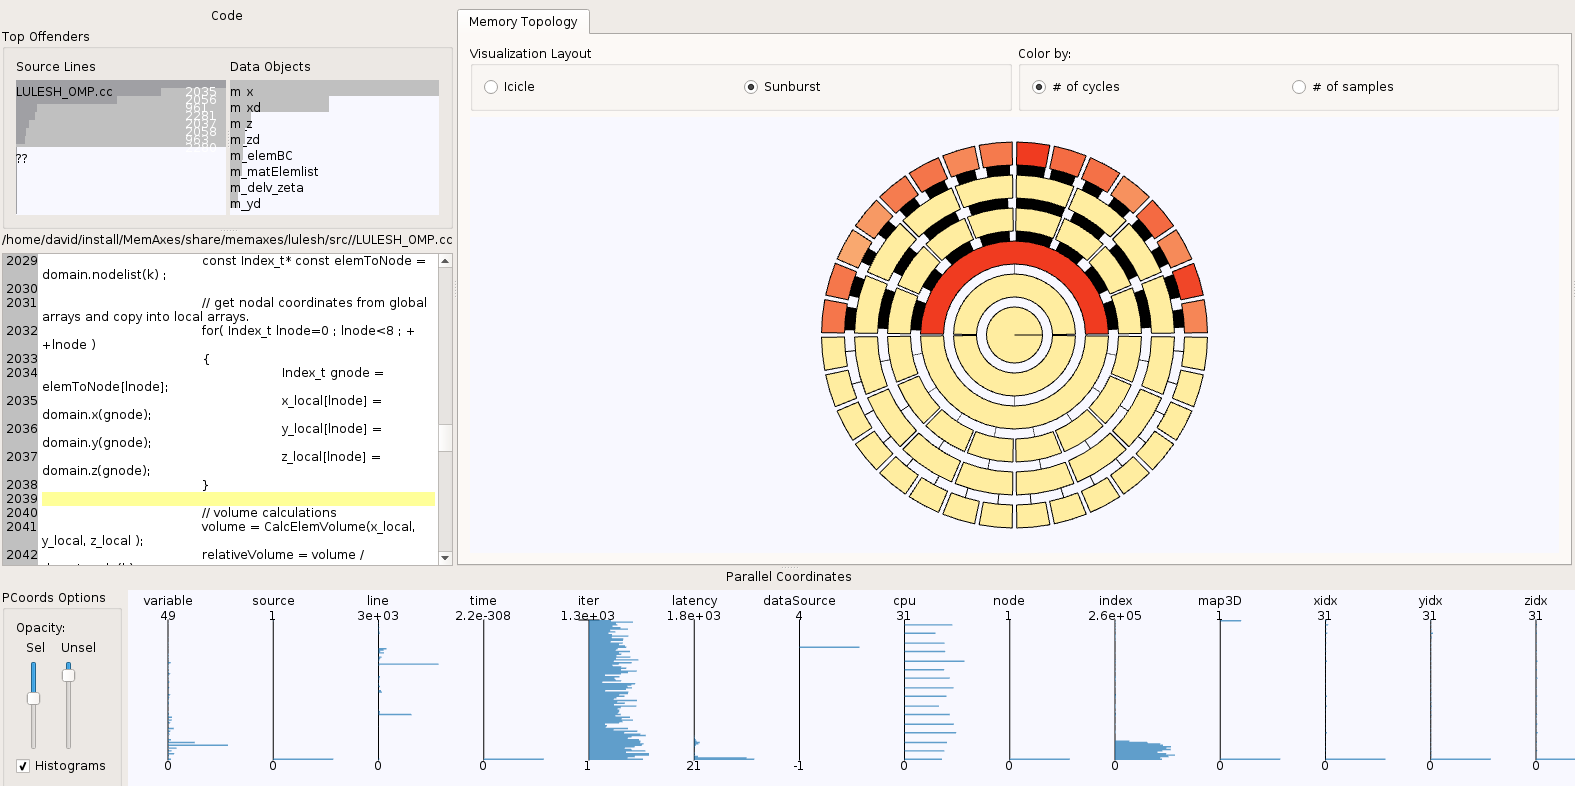
\includegraphics[width=\linewidth]{memAxes.png}
    \caption[Screenshot from MemAxes.]{Screenshot from MemAxes on the example data trace provided with the
    tool.}
    \label{fig:memaxes}
\end{figure}

Finally, \gls{MemAxes}~\cite{Gimenez14Dissecting}, which is the visualization tool for \gls{Mitos}, provide a unified view of the trace.
This view, presented in \fig{memaxes}, correlates the information collected in the samples (bottom pane) with the architecture (middle pane) and the source code and data structures (left pane).
It enables to do some selection on any part of the visualization to focus on some code or a NUMA node etc.
Furthermore, Husain et al.~\cite{Husain15Relating} have recently added a layer to \gls{MemAxes} that enable to trace simulations and link the simulation visualization to \gls{MemAxes}.
Still, this visualization does not show sharing pattern or access patterns, it only helps identifying the lines of code and data structures responsible for the bad performances (hotspots)
As a result, the user still has to correlate the samples information to understand the nature of the issue and how to fix it.

\section{Conclusions}
\label{sec:mem-cncl}

The memory subsystems have became more and more complex over the last few decades.
As a result, the way a program allocates and access its memory has a significant impact on the performances.
Eventually, a developer looking for performances must consider the memory access patterns of its application.
Therefore a tool able to collect a memory trace and to display accesses and sharing patterns would be useful for performance optimization.

Most existing memory trace collection tools consider the memory as a monolithic entity and only provide global information such as the bandwidth.
Some tools provide more detailed memory traces.
Nevertheless, they rely either on  hardware based sampling in which case the resulting trace only shows a small subset of the memory, or on hardware modifications and are thus not usable by real life developers.

When it comes to visualizing these traces, many techniques were developed to identify precisely in the code and data structures where performances are suboptimal.
Yet, most of the existing tools are not able to show memory patterns of any kind.
A few advanced tools picture the number of accesses per data structure and per thread or the number of remote accesses per page.
Still this is not sufficient to understand precisely sharing patterns or memory access patterns.

To conclude we need both to collect precise memory traces and to present them to the user in a comprehensive way that enable identification of sharing and access patterns.
% vim: et si sta lbr  sw=4 ts=4 spelllang=en_us
